
% Default to the notebook output style

    


% Inherit from the specified cell style.




    
\documentclass[11pt]{article}

    
    
    \usepackage[T1]{fontenc}
    % Nicer default font (+ math font) than Computer Modern for most use cases
    \usepackage{mathpazo}

    % Basic figure setup, for now with no caption control since it's done
    % automatically by Pandoc (which extracts ![](path) syntax from Markdown).
    \usepackage{graphicx}
    % We will generate all images so they have a width \maxwidth. This means
    % that they will get their normal width if they fit onto the page, but
    % are scaled down if they would overflow the margins.
    \makeatletter
    \def\maxwidth{\ifdim\Gin@nat@width>\linewidth\linewidth
    \else\Gin@nat@width\fi}
    \makeatother
    \let\Oldincludegraphics\includegraphics
    % Set max figure width to be 80% of text width, for now hardcoded.
    \renewcommand{\includegraphics}[1]{\Oldincludegraphics[width=.8\maxwidth]{#1}}
    % Ensure that by default, figures have no caption (until we provide a
    % proper Figure object with a Caption API and a way to capture that
    % in the conversion process - todo).
    \usepackage{caption}
    \DeclareCaptionLabelFormat{nolabel}{}
    \captionsetup{labelformat=nolabel}

    \usepackage{adjustbox} % Used to constrain images to a maximum size 
    \usepackage{xcolor} % Allow colors to be defined
    \usepackage{enumerate} % Needed for markdown enumerations to work
    \usepackage{geometry} % Used to adjust the document margins
    \usepackage{amsmath} % Equations
    \usepackage{amssymb} % Equations
    \usepackage{textcomp} % defines textquotesingle
    % Hack from http://tex.stackexchange.com/a/47451/13684:
    \AtBeginDocument{%
        \def\PYZsq{\textquotesingle}% Upright quotes in Pygmentized code
    }
    \usepackage{upquote} % Upright quotes for verbatim code
    \usepackage{eurosym} % defines \euro
    \usepackage[mathletters]{ucs} % Extended unicode (utf-8) support
    \usepackage[utf8x]{inputenc} % Allow utf-8 characters in the tex document
    \usepackage{fancyvrb} % verbatim replacement that allows latex
    \usepackage{grffile} % extends the file name processing of package graphics 
                         % to support a larger range 
    % The hyperref package gives us a pdf with properly built
    % internal navigation ('pdf bookmarks' for the table of contents,
    % internal cross-reference links, web links for URLs, etc.)
    \usepackage{hyperref}
    \usepackage{longtable} % longtable support required by pandoc >1.10
    \usepackage{booktabs}  % table support for pandoc > 1.12.2
    \usepackage[inline]{enumitem} % IRkernel/repr support (it uses the enumerate* environment)
    \usepackage[normalem]{ulem} % ulem is needed to support strikethroughs (\sout)
                                % normalem makes italics be italics, not underlines
    

    
    
    % Colors for the hyperref package
    \definecolor{urlcolor}{rgb}{0,.145,.698}
    \definecolor{linkcolor}{rgb}{.71,0.21,0.01}
    \definecolor{citecolor}{rgb}{.12,.54,.11}

    % ANSI colors
    \definecolor{ansi-black}{HTML}{3E424D}
    \definecolor{ansi-black-intense}{HTML}{282C36}
    \definecolor{ansi-red}{HTML}{E75C58}
    \definecolor{ansi-red-intense}{HTML}{B22B31}
    \definecolor{ansi-green}{HTML}{00A250}
    \definecolor{ansi-green-intense}{HTML}{007427}
    \definecolor{ansi-yellow}{HTML}{DDB62B}
    \definecolor{ansi-yellow-intense}{HTML}{B27D12}
    \definecolor{ansi-blue}{HTML}{208FFB}
    \definecolor{ansi-blue-intense}{HTML}{0065CA}
    \definecolor{ansi-magenta}{HTML}{D160C4}
    \definecolor{ansi-magenta-intense}{HTML}{A03196}
    \definecolor{ansi-cyan}{HTML}{60C6C8}
    \definecolor{ansi-cyan-intense}{HTML}{258F8F}
    \definecolor{ansi-white}{HTML}{C5C1B4}
    \definecolor{ansi-white-intense}{HTML}{A1A6B2}

    % commands and environments needed by pandoc snippets
    % extracted from the output of `pandoc -s`
    \providecommand{\tightlist}{%
      \setlength{\itemsep}{0pt}\setlength{\parskip}{0pt}}
    \DefineVerbatimEnvironment{Highlighting}{Verbatim}{commandchars=\\\{\}}
    % Add ',fontsize=\small' for more characters per line
    \newenvironment{Shaded}{}{}
    \newcommand{\KeywordTok}[1]{\textcolor[rgb]{0.00,0.44,0.13}{\textbf{{#1}}}}
    \newcommand{\DataTypeTok}[1]{\textcolor[rgb]{0.56,0.13,0.00}{{#1}}}
    \newcommand{\DecValTok}[1]{\textcolor[rgb]{0.25,0.63,0.44}{{#1}}}
    \newcommand{\BaseNTok}[1]{\textcolor[rgb]{0.25,0.63,0.44}{{#1}}}
    \newcommand{\FloatTok}[1]{\textcolor[rgb]{0.25,0.63,0.44}{{#1}}}
    \newcommand{\CharTok}[1]{\textcolor[rgb]{0.25,0.44,0.63}{{#1}}}
    \newcommand{\StringTok}[1]{\textcolor[rgb]{0.25,0.44,0.63}{{#1}}}
    \newcommand{\CommentTok}[1]{\textcolor[rgb]{0.38,0.63,0.69}{\textit{{#1}}}}
    \newcommand{\OtherTok}[1]{\textcolor[rgb]{0.00,0.44,0.13}{{#1}}}
    \newcommand{\AlertTok}[1]{\textcolor[rgb]{1.00,0.00,0.00}{\textbf{{#1}}}}
    \newcommand{\FunctionTok}[1]{\textcolor[rgb]{0.02,0.16,0.49}{{#1}}}
    \newcommand{\RegionMarkerTok}[1]{{#1}}
    \newcommand{\ErrorTok}[1]{\textcolor[rgb]{1.00,0.00,0.00}{\textbf{{#1}}}}
    \newcommand{\NormalTok}[1]{{#1}}
    
    % Additional commands for more recent versions of Pandoc
    \newcommand{\ConstantTok}[1]{\textcolor[rgb]{0.53,0.00,0.00}{{#1}}}
    \newcommand{\SpecialCharTok}[1]{\textcolor[rgb]{0.25,0.44,0.63}{{#1}}}
    \newcommand{\VerbatimStringTok}[1]{\textcolor[rgb]{0.25,0.44,0.63}{{#1}}}
    \newcommand{\SpecialStringTok}[1]{\textcolor[rgb]{0.73,0.40,0.53}{{#1}}}
    \newcommand{\ImportTok}[1]{{#1}}
    \newcommand{\DocumentationTok}[1]{\textcolor[rgb]{0.73,0.13,0.13}{\textit{{#1}}}}
    \newcommand{\AnnotationTok}[1]{\textcolor[rgb]{0.38,0.63,0.69}{\textbf{\textit{{#1}}}}}
    \newcommand{\CommentVarTok}[1]{\textcolor[rgb]{0.38,0.63,0.69}{\textbf{\textit{{#1}}}}}
    \newcommand{\VariableTok}[1]{\textcolor[rgb]{0.10,0.09,0.49}{{#1}}}
    \newcommand{\ControlFlowTok}[1]{\textcolor[rgb]{0.00,0.44,0.13}{\textbf{{#1}}}}
    \newcommand{\OperatorTok}[1]{\textcolor[rgb]{0.40,0.40,0.40}{{#1}}}
    \newcommand{\BuiltInTok}[1]{{#1}}
    \newcommand{\ExtensionTok}[1]{{#1}}
    \newcommand{\PreprocessorTok}[1]{\textcolor[rgb]{0.74,0.48,0.00}{{#1}}}
    \newcommand{\AttributeTok}[1]{\textcolor[rgb]{0.49,0.56,0.16}{{#1}}}
    \newcommand{\InformationTok}[1]{\textcolor[rgb]{0.38,0.63,0.69}{\textbf{\textit{{#1}}}}}
    \newcommand{\WarningTok}[1]{\textcolor[rgb]{0.38,0.63,0.69}{\textbf{\textit{{#1}}}}}
    
    
    % Define a nice break command that doesn't care if a line doesn't already
    % exist.
    \def\br{\hspace*{\fill} \\* }
    % Math Jax compatability definitions
    \def\gt{>}
    \def\lt{<}
    % Document parameters
    \title{HW1}
    
    
    

    % Pygments definitions
    
\makeatletter
\def\PY@reset{\let\PY@it=\relax \let\PY@bf=\relax%
    \let\PY@ul=\relax \let\PY@tc=\relax%
    \let\PY@bc=\relax \let\PY@ff=\relax}
\def\PY@tok#1{\csname PY@tok@#1\endcsname}
\def\PY@toks#1+{\ifx\relax#1\empty\else%
    \PY@tok{#1}\expandafter\PY@toks\fi}
\def\PY@do#1{\PY@bc{\PY@tc{\PY@ul{%
    \PY@it{\PY@bf{\PY@ff{#1}}}}}}}
\def\PY#1#2{\PY@reset\PY@toks#1+\relax+\PY@do{#2}}

\expandafter\def\csname PY@tok@w\endcsname{\def\PY@tc##1{\textcolor[rgb]{0.73,0.73,0.73}{##1}}}
\expandafter\def\csname PY@tok@c\endcsname{\let\PY@it=\textit\def\PY@tc##1{\textcolor[rgb]{0.25,0.50,0.50}{##1}}}
\expandafter\def\csname PY@tok@cp\endcsname{\def\PY@tc##1{\textcolor[rgb]{0.74,0.48,0.00}{##1}}}
\expandafter\def\csname PY@tok@k\endcsname{\let\PY@bf=\textbf\def\PY@tc##1{\textcolor[rgb]{0.00,0.50,0.00}{##1}}}
\expandafter\def\csname PY@tok@kp\endcsname{\def\PY@tc##1{\textcolor[rgb]{0.00,0.50,0.00}{##1}}}
\expandafter\def\csname PY@tok@kt\endcsname{\def\PY@tc##1{\textcolor[rgb]{0.69,0.00,0.25}{##1}}}
\expandafter\def\csname PY@tok@o\endcsname{\def\PY@tc##1{\textcolor[rgb]{0.40,0.40,0.40}{##1}}}
\expandafter\def\csname PY@tok@ow\endcsname{\let\PY@bf=\textbf\def\PY@tc##1{\textcolor[rgb]{0.67,0.13,1.00}{##1}}}
\expandafter\def\csname PY@tok@nb\endcsname{\def\PY@tc##1{\textcolor[rgb]{0.00,0.50,0.00}{##1}}}
\expandafter\def\csname PY@tok@nf\endcsname{\def\PY@tc##1{\textcolor[rgb]{0.00,0.00,1.00}{##1}}}
\expandafter\def\csname PY@tok@nc\endcsname{\let\PY@bf=\textbf\def\PY@tc##1{\textcolor[rgb]{0.00,0.00,1.00}{##1}}}
\expandafter\def\csname PY@tok@nn\endcsname{\let\PY@bf=\textbf\def\PY@tc##1{\textcolor[rgb]{0.00,0.00,1.00}{##1}}}
\expandafter\def\csname PY@tok@ne\endcsname{\let\PY@bf=\textbf\def\PY@tc##1{\textcolor[rgb]{0.82,0.25,0.23}{##1}}}
\expandafter\def\csname PY@tok@nv\endcsname{\def\PY@tc##1{\textcolor[rgb]{0.10,0.09,0.49}{##1}}}
\expandafter\def\csname PY@tok@no\endcsname{\def\PY@tc##1{\textcolor[rgb]{0.53,0.00,0.00}{##1}}}
\expandafter\def\csname PY@tok@nl\endcsname{\def\PY@tc##1{\textcolor[rgb]{0.63,0.63,0.00}{##1}}}
\expandafter\def\csname PY@tok@ni\endcsname{\let\PY@bf=\textbf\def\PY@tc##1{\textcolor[rgb]{0.60,0.60,0.60}{##1}}}
\expandafter\def\csname PY@tok@na\endcsname{\def\PY@tc##1{\textcolor[rgb]{0.49,0.56,0.16}{##1}}}
\expandafter\def\csname PY@tok@nt\endcsname{\let\PY@bf=\textbf\def\PY@tc##1{\textcolor[rgb]{0.00,0.50,0.00}{##1}}}
\expandafter\def\csname PY@tok@nd\endcsname{\def\PY@tc##1{\textcolor[rgb]{0.67,0.13,1.00}{##1}}}
\expandafter\def\csname PY@tok@s\endcsname{\def\PY@tc##1{\textcolor[rgb]{0.73,0.13,0.13}{##1}}}
\expandafter\def\csname PY@tok@sd\endcsname{\let\PY@it=\textit\def\PY@tc##1{\textcolor[rgb]{0.73,0.13,0.13}{##1}}}
\expandafter\def\csname PY@tok@si\endcsname{\let\PY@bf=\textbf\def\PY@tc##1{\textcolor[rgb]{0.73,0.40,0.53}{##1}}}
\expandafter\def\csname PY@tok@se\endcsname{\let\PY@bf=\textbf\def\PY@tc##1{\textcolor[rgb]{0.73,0.40,0.13}{##1}}}
\expandafter\def\csname PY@tok@sr\endcsname{\def\PY@tc##1{\textcolor[rgb]{0.73,0.40,0.53}{##1}}}
\expandafter\def\csname PY@tok@ss\endcsname{\def\PY@tc##1{\textcolor[rgb]{0.10,0.09,0.49}{##1}}}
\expandafter\def\csname PY@tok@sx\endcsname{\def\PY@tc##1{\textcolor[rgb]{0.00,0.50,0.00}{##1}}}
\expandafter\def\csname PY@tok@m\endcsname{\def\PY@tc##1{\textcolor[rgb]{0.40,0.40,0.40}{##1}}}
\expandafter\def\csname PY@tok@gh\endcsname{\let\PY@bf=\textbf\def\PY@tc##1{\textcolor[rgb]{0.00,0.00,0.50}{##1}}}
\expandafter\def\csname PY@tok@gu\endcsname{\let\PY@bf=\textbf\def\PY@tc##1{\textcolor[rgb]{0.50,0.00,0.50}{##1}}}
\expandafter\def\csname PY@tok@gd\endcsname{\def\PY@tc##1{\textcolor[rgb]{0.63,0.00,0.00}{##1}}}
\expandafter\def\csname PY@tok@gi\endcsname{\def\PY@tc##1{\textcolor[rgb]{0.00,0.63,0.00}{##1}}}
\expandafter\def\csname PY@tok@gr\endcsname{\def\PY@tc##1{\textcolor[rgb]{1.00,0.00,0.00}{##1}}}
\expandafter\def\csname PY@tok@ge\endcsname{\let\PY@it=\textit}
\expandafter\def\csname PY@tok@gs\endcsname{\let\PY@bf=\textbf}
\expandafter\def\csname PY@tok@gp\endcsname{\let\PY@bf=\textbf\def\PY@tc##1{\textcolor[rgb]{0.00,0.00,0.50}{##1}}}
\expandafter\def\csname PY@tok@go\endcsname{\def\PY@tc##1{\textcolor[rgb]{0.53,0.53,0.53}{##1}}}
\expandafter\def\csname PY@tok@gt\endcsname{\def\PY@tc##1{\textcolor[rgb]{0.00,0.27,0.87}{##1}}}
\expandafter\def\csname PY@tok@err\endcsname{\def\PY@bc##1{\setlength{\fboxsep}{0pt}\fcolorbox[rgb]{1.00,0.00,0.00}{1,1,1}{\strut ##1}}}
\expandafter\def\csname PY@tok@kc\endcsname{\let\PY@bf=\textbf\def\PY@tc##1{\textcolor[rgb]{0.00,0.50,0.00}{##1}}}
\expandafter\def\csname PY@tok@kd\endcsname{\let\PY@bf=\textbf\def\PY@tc##1{\textcolor[rgb]{0.00,0.50,0.00}{##1}}}
\expandafter\def\csname PY@tok@kn\endcsname{\let\PY@bf=\textbf\def\PY@tc##1{\textcolor[rgb]{0.00,0.50,0.00}{##1}}}
\expandafter\def\csname PY@tok@kr\endcsname{\let\PY@bf=\textbf\def\PY@tc##1{\textcolor[rgb]{0.00,0.50,0.00}{##1}}}
\expandafter\def\csname PY@tok@bp\endcsname{\def\PY@tc##1{\textcolor[rgb]{0.00,0.50,0.00}{##1}}}
\expandafter\def\csname PY@tok@fm\endcsname{\def\PY@tc##1{\textcolor[rgb]{0.00,0.00,1.00}{##1}}}
\expandafter\def\csname PY@tok@vc\endcsname{\def\PY@tc##1{\textcolor[rgb]{0.10,0.09,0.49}{##1}}}
\expandafter\def\csname PY@tok@vg\endcsname{\def\PY@tc##1{\textcolor[rgb]{0.10,0.09,0.49}{##1}}}
\expandafter\def\csname PY@tok@vi\endcsname{\def\PY@tc##1{\textcolor[rgb]{0.10,0.09,0.49}{##1}}}
\expandafter\def\csname PY@tok@vm\endcsname{\def\PY@tc##1{\textcolor[rgb]{0.10,0.09,0.49}{##1}}}
\expandafter\def\csname PY@tok@sa\endcsname{\def\PY@tc##1{\textcolor[rgb]{0.73,0.13,0.13}{##1}}}
\expandafter\def\csname PY@tok@sb\endcsname{\def\PY@tc##1{\textcolor[rgb]{0.73,0.13,0.13}{##1}}}
\expandafter\def\csname PY@tok@sc\endcsname{\def\PY@tc##1{\textcolor[rgb]{0.73,0.13,0.13}{##1}}}
\expandafter\def\csname PY@tok@dl\endcsname{\def\PY@tc##1{\textcolor[rgb]{0.73,0.13,0.13}{##1}}}
\expandafter\def\csname PY@tok@s2\endcsname{\def\PY@tc##1{\textcolor[rgb]{0.73,0.13,0.13}{##1}}}
\expandafter\def\csname PY@tok@sh\endcsname{\def\PY@tc##1{\textcolor[rgb]{0.73,0.13,0.13}{##1}}}
\expandafter\def\csname PY@tok@s1\endcsname{\def\PY@tc##1{\textcolor[rgb]{0.73,0.13,0.13}{##1}}}
\expandafter\def\csname PY@tok@mb\endcsname{\def\PY@tc##1{\textcolor[rgb]{0.40,0.40,0.40}{##1}}}
\expandafter\def\csname PY@tok@mf\endcsname{\def\PY@tc##1{\textcolor[rgb]{0.40,0.40,0.40}{##1}}}
\expandafter\def\csname PY@tok@mh\endcsname{\def\PY@tc##1{\textcolor[rgb]{0.40,0.40,0.40}{##1}}}
\expandafter\def\csname PY@tok@mi\endcsname{\def\PY@tc##1{\textcolor[rgb]{0.40,0.40,0.40}{##1}}}
\expandafter\def\csname PY@tok@il\endcsname{\def\PY@tc##1{\textcolor[rgb]{0.40,0.40,0.40}{##1}}}
\expandafter\def\csname PY@tok@mo\endcsname{\def\PY@tc##1{\textcolor[rgb]{0.40,0.40,0.40}{##1}}}
\expandafter\def\csname PY@tok@ch\endcsname{\let\PY@it=\textit\def\PY@tc##1{\textcolor[rgb]{0.25,0.50,0.50}{##1}}}
\expandafter\def\csname PY@tok@cm\endcsname{\let\PY@it=\textit\def\PY@tc##1{\textcolor[rgb]{0.25,0.50,0.50}{##1}}}
\expandafter\def\csname PY@tok@cpf\endcsname{\let\PY@it=\textit\def\PY@tc##1{\textcolor[rgb]{0.25,0.50,0.50}{##1}}}
\expandafter\def\csname PY@tok@c1\endcsname{\let\PY@it=\textit\def\PY@tc##1{\textcolor[rgb]{0.25,0.50,0.50}{##1}}}
\expandafter\def\csname PY@tok@cs\endcsname{\let\PY@it=\textit\def\PY@tc##1{\textcolor[rgb]{0.25,0.50,0.50}{##1}}}

\def\PYZbs{\char`\\}
\def\PYZus{\char`\_}
\def\PYZob{\char`\{}
\def\PYZcb{\char`\}}
\def\PYZca{\char`\^}
\def\PYZam{\char`\&}
\def\PYZlt{\char`\<}
\def\PYZgt{\char`\>}
\def\PYZsh{\char`\#}
\def\PYZpc{\char`\%}
\def\PYZdl{\char`\$}
\def\PYZhy{\char`\-}
\def\PYZsq{\char`\'}
\def\PYZdq{\char`\"}
\def\PYZti{\char`\~}
% for compatibility with earlier versions
\def\PYZat{@}
\def\PYZlb{[}
\def\PYZrb{]}
\makeatother


    % Exact colors from NB
    \definecolor{incolor}{rgb}{0.0, 0.0, 0.5}
    \definecolor{outcolor}{rgb}{0.545, 0.0, 0.0}



    
    % Prevent overflowing lines due to hard-to-break entities
    \sloppy 
    % Setup hyperref package
    \hypersetup{
      breaklinks=true,  % so long urls are correctly broken across lines
      colorlinks=true,
      urlcolor=urlcolor,
      linkcolor=linkcolor,
      citecolor=citecolor,
      }
    % Slightly bigger margins than the latex defaults
    
    \geometry{verbose,tmargin=1in,bmargin=1in,lmargin=1in,rmargin=1in}
    
    

    \begin{document}
    
    
    \maketitle
    
    

    
    \hypertarget{digital-image-processing---hw1---98722278---mohammad-doosti-lakhani}{%
\section{Digital Image Processing - HW1 - 98722278 - Mohammad Doosti
Lakhani}\label{digital-image-processing---hw1---98722278---mohammad-doosti-lakhani}}

In this notebook, I have solved the assignment's problems which are as
follows:

\begin{enumerate}
\def\labelenumi{\arabic{enumi}.}
\tightlist
\item
  Explain an idea which can be used in a start-up which uses computer
  vision. No need to expalin the algorithms and how-tos.
\item
  What is ``Shutter Speed'' feature in cameras and how it can impact on
  image quality?
\item
  Implement the \texttt{equalize\_hist1} and \texttt{equalize\_hist2}
  functions regarding following steps:

  \begin{enumerate}
  \def\labelenumii{\arabic{enumii}.}
  \tightlist
  \item
    Implement \emph{histogram equalization} via \textbf{open\_cv} in
    \texttt{equalize\_hist1}
  \item
    Implement \emph{histogram equalization} based on the what have been
    taught in slides in \texttt{equalize\_hist2}
  \item
    Plot the \texttt{T} function
  \item
    Plot the histogram of images before equalization and after it.
  \item
    Explain the differences
  \end{enumerate}
\end{enumerate}

    \hypertarget{explain-an-idea-which-uses-computer-vision}{%
\subsection{1. Explain an idea which uses computer
vision}\label{explain-an-idea-which-uses-computer-vision}}

In this section, I want to talk about the idea so-called \emph{Lie
detection based on body language}. This explanation consists of these
parts: 1.
Section \ref{22lie-detection-based-on-body-language22-intorduction} 2.
Section \ref{usage} 3. Section \ref{references}

\hypertarget{lie-detection-based-on-body-language-intorduction}{%
\subsubsection{1.1 ``Lie Detection Based on Body Language''
Intorduction}\label{lie-detection-based-on-body-language-intorduction}}

I would like to kick of by mentioning the point that as all of us know,
when people attempt to lie (orally), they illustrate some signs on their
bodies particularly on their faces or hands. In this report, I will
focus on the simplified one which only focuses on children's hands and
faces' major signs, for instance blinking abnormally to help parents
detect the lies and help their children to overcome the hardship without
losing the control of circumstances.

\hypertarget{usage}{%
\subsubsection{1.2 Usage}\label{usage}}

Based on what I have mentioned in the intro section, we can say a group
of signs in most cases can lead to a lie confidently1. And all of those
signs have been extracted by experts like agents in police departments
so they are all reliable features. For a simple demonstration, we can
say the children who start scratching their noses or the back of their
heads at the time of talking to their parents or teachers, mostly they
are trying to deceive their contacts.2.

This proposal has aimed these facts to create a automated system for
parents and teachers to capture images while speaking to the children
and detect lies. On top of that, parents or teachers will be able to
manage the situation and try to understand why their chidlren or
students are trying to lie to them. One of the possible causes of lying
by children could be feeling insecure about their own abilities. In this
kind of situation, the teacher or parent will notice that using this
system and instead of putting more pressure on the child or speaking in
the way that may cause more fear, try to conciliate and help children by
giving them confidence3.

The scale of capturing can be used in three level: 1. Capturing the
whole body and focusing only on prominent body language characteristics
2. Capturing face/hands to explore the possiblities using more detailed
features. 3. Capturing eye/lips/shaking and heat level (not considered
as body language but very usefull) to expand the feature pool.

\hypertarget{references}{%
\subsubsection{1.3 References}\label{references}}

\begin{enumerate}
\def\labelenumi{\arabic{enumi}.}
\tightlist
\item
  \href{https://www.amazon.com/Human-Lie-Detection-Body-Language/dp/1482040239}{Human
  Lie Detection and Body Language 101: Your Guide to Reading People's
  Nonverbal Behavior - Vanessa Van Edwards}
\item
  \href{https://medium.com/@101/how-to-detect-lies-body-language-5a184e90337b\#targetText=The\%20Nose\%20Touch\&targetText=However\%2C\%20the\%20hand\%20is\%20quickly,satisfied\%20with\%20rubbing\%20or\%20scratching.}{How
  to detect lies body language - Nick Babich on Medium}
\item
  \href{https://www.ncbi.nlm.nih.gov/pmc/articles/PMC3483871/}{Social
  and Cognitive Correlates of Children's Lying Behavior - Victoria
  Talwar and Kang Lee}
\end{enumerate}

    \hypertarget{the-impact-of-shutter-speed-on-the-quality-of-captured-images-via-camera}{%
\subsection{2. The Impact of ``Shutter Speed'' On The Quality of
Captured Images via
Camera}\label{the-impact-of-shutter-speed-on-the-quality-of-captured-images-via-camera}}

In this section, questions such as \emph{what is shutter speed},
\emph{what is its impact} will be answered in the following sections: 1.
Shutter Intro 2. Shutter Speed and Its Effects 1. Exposure (Brightness)
2. Motion 3. Final Words 4. References

\hypertarget{shutter-intro}{%
\subsubsection{2.1 Shutter Intro}\label{shutter-intro}}

As we know, cameras take photos by exposing their digital sensors to the
light. Shutter, as its name illustrates, is a barrier that keeps the
light out from the camera's sensors and it opens when you try to take
photo by pressing \emph{shutter} button on your camera and closes after
the photo has been taken which means after closing, sensors are no
longer exposed to the light.

\hypertarget{shutter-speed}{%
\subsubsection{2.2 Shutter Speed}\label{shutter-speed}}

Based on what we read in previous section, camera only take photo when
its shutter is open, so now a parameter emerges; the
\emph{\textbf{speeed}}. The shutter speed is the time it takes from
opening shutter and exposing sensors to the light till closing it and it
is categorized into two major types: 1. Fast: Conventionally a small
fraction of a second for instance 1/100th second or 1/200th second to
1/4000th second. 2. Slow Conventionally more than a second for instance
1, 5, even 30 or a few mintues depends on the task.

These spectrum of speeds have completely different effect on the taken
photo from making it brighter or darker or even blury or sharp. Having a
slow shutter means more exposure to the light and in case of brightness,
the sensors would gain more light and vice versa. Meanwhile, if object
moves, slow shutter means blury images and vice versa. These will be
discussed in the following section more detailed.

\hypertarget{a-exposure}{%
\paragraph{2.2.A Exposure}\label{a-exposure}}

Let say object and subjects are still and we use slow shutter. In this
situation, the sensors have more time to absorb the light and it means
we will have brighter images. It is very usefull in dark environments
specially night scenes. But you need to consider that exposing too much
to light means a fully bright image of the scene called
\emph{overexposed}, on the other hand, have a quick shutter in dark
environment will give a dark image. But shutter speed is not the only
factor that impacts the brightness, others are \textbf{ISO} and
\textbf{Aperture} which we do not discuss here.

Below is an image that portrays the effect of the shutter speed on the
brightness:

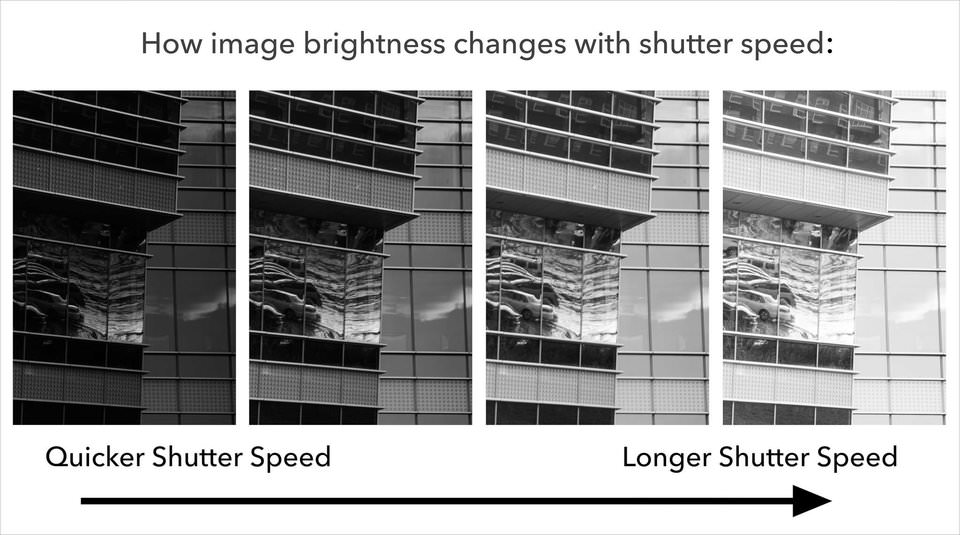
\includegraphics{wiki/exposure1.jpg} Photo:
\href{https://photographylife.com}{photographylife.com}

\hypertarget{b-motion}{%
\paragraph{2.2.B Motion}\label{b-motion}}

In this section, the being still constraint has been removed which means
the subjects can move at different speeds while the shutter is open (the
camera itself can move too but the effect is almost same). It is known
to us that the image could be created when light reflects from the
objects and if let say point \texttt{x}, exposes to different sensors of
camera, its effect will be all there so moving an object while the
camera is taking photo means different points of the objects will be
reflected on many different sensors not just one and it causes a blury
image as we have seen this effect in \emph{rolling shutter} or
\emph{global shutter} designs. Actually, it is all about time and
because we have a slow shutter, the output will be blury. Note that if
nothing moves, it will not be blury, only objects that moves create
blury effect in the path they move along and many photographer use these
may seem drawback as a upside and create fascinating images that only a
part of a image is blury which is called \emph{\textbf{Motion Blur}}.
Below is the example:

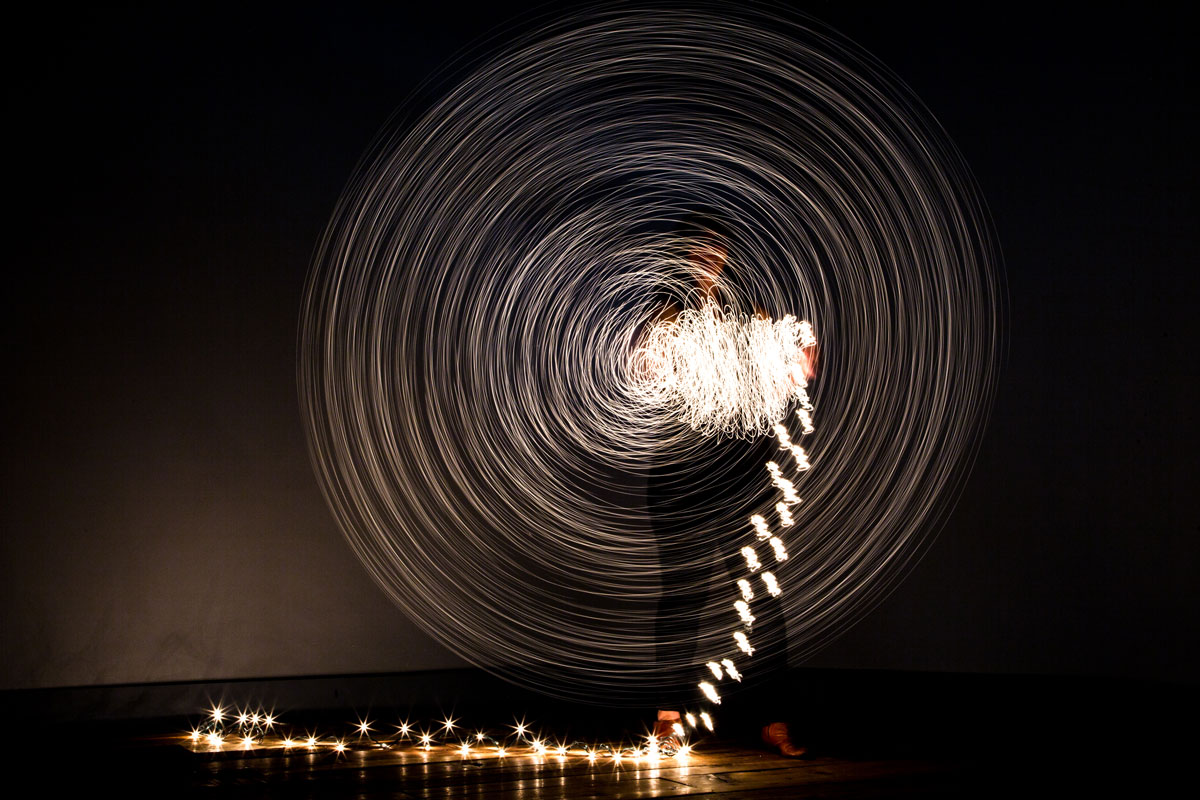
\includegraphics{wiki/motionblur1.jpg} Photo: Casey Cosley

On the other hand, if we use a fast shutter, no matter object are moving
(but it is important how fast they are) we can achieve a stabilized and
still image of the moving object without introducing blur effect. The
reason is when shutter closes very fast, each point of the object only
reflect on a very small number of sensors and it seems to that objects
are stand. One point that will not be waste of time to mention is that
if camera and the objects move at the same pace, the image will not be
blury but it is a little bit tricky to acquire. Below is an example of
fast shutter on moving object:

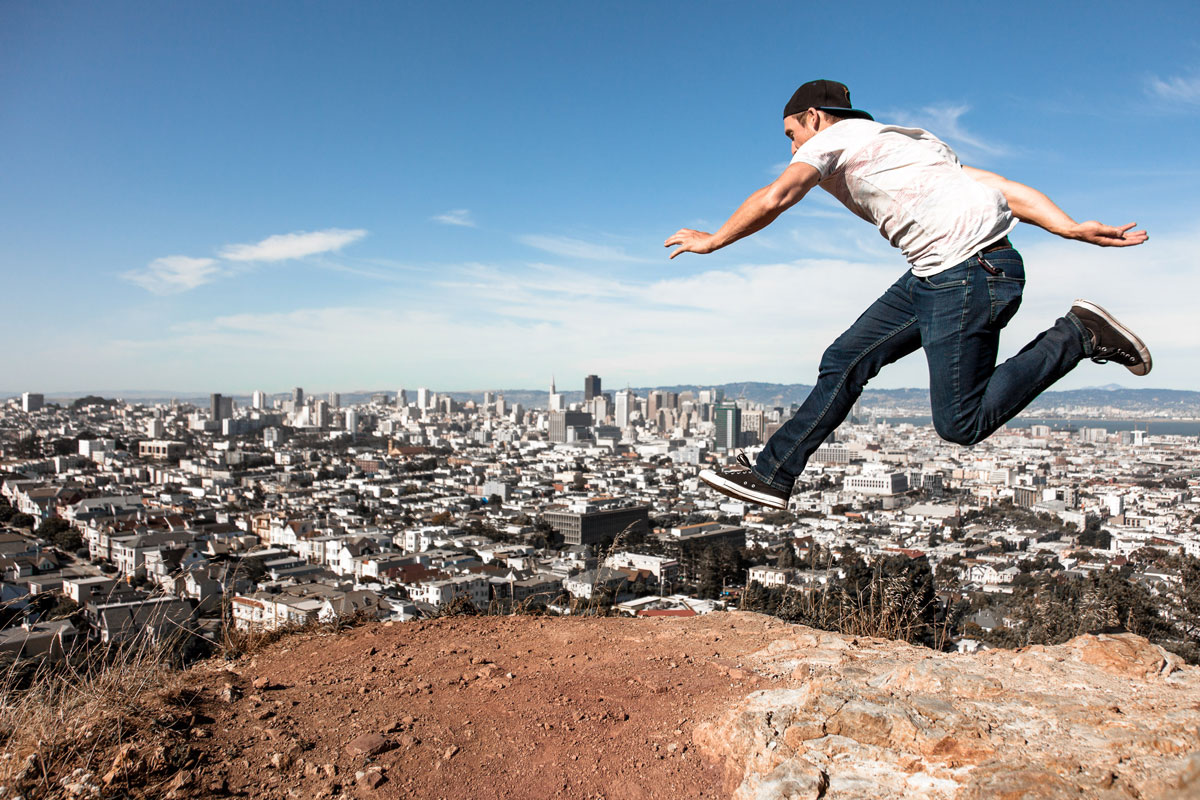
\includegraphics{wiki/freezemotion1.jpg} Photo: Matt McMonagle

To finish this section, a image that demonstrates the differences
between shutter speed and blur effect is great.

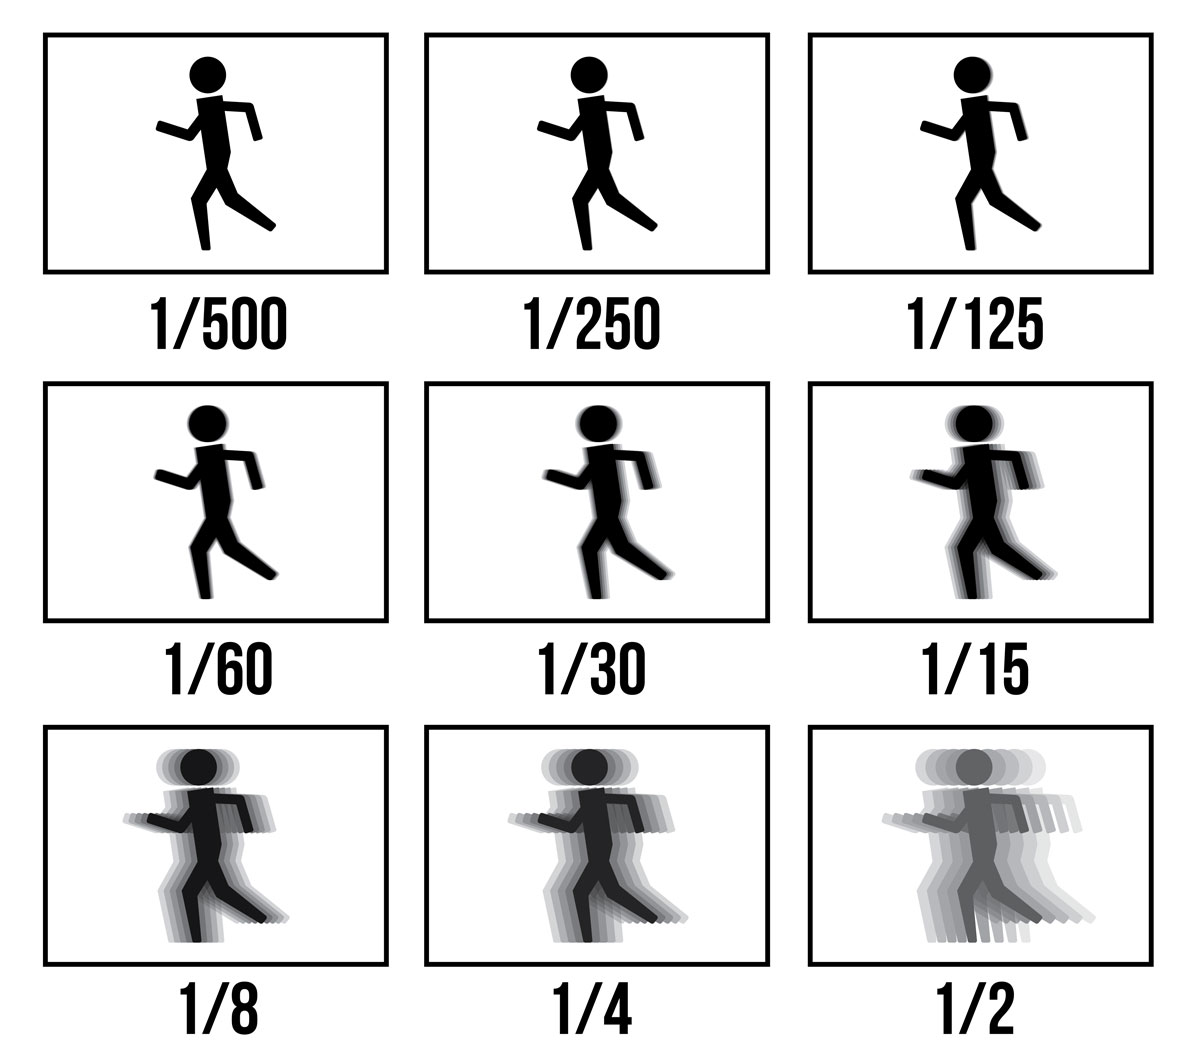
\includegraphics{wiki/motionblur2.jpg} Photo:
\href{https://creativelive.com}{creativelive.com}

\hypertarget{final-words}{%
\subsubsection{2.3 Final Words}\label{final-words}}

Even though at first sight slow shutter may seem as a drawback at taking
photos, but it can help to achieve spectacular presentation of a scene.
Although it may help create enticing images, exposure is the other
effect that need to be dealt because of the low speed of the shutter.

\hypertarget{references}{%
\subsubsection{2.4 References}\label{references}}

\begin{enumerate}
\def\labelenumi{\arabic{enumi}.}
\tightlist
\item
  \href{https://www.creativelive.com/photography-guides/what-is-shutter-speed}{The
  Ultimate Guide To Learning Photography: Shutter Speed -
  creativelive.com}
\item
  \href{https://photographylife.com/what-is-shutter-speed-in-photography}{Introduction
  to Shutter Speed in Photography - Nasim Mansurov}
\end{enumerate}

    \hypertarget{histogram-equalization}{%
\subsection{3 Histogram Equalization}\label{histogram-equalization}}

In this section, the usage of \emph{\textbf{histogram-equalization}}
using \textbf{open-cv} and out implementation will be demonstrated. This
secions consistes of following: 1. \texttt{equalize\_hist1} - open\_cv
2. \texttt{equalize\_hist2} - Ours 1. \texttt{histogram} 2.
\texttt{equalize\_hist2} 3. \texttt{T} Plot

    \begin{Verbatim}[commandchars=\\\{\}]
{\color{incolor}In [{\color{incolor}38}]:} \PY{c+c1}{\PYZsh{} necessary variables}
         \PY{k+kn}{import} \PY{n+nn}{os}
         \PY{k+kn}{import} \PY{n+nn}{cv2}
         \PY{k+kn}{import} \PY{n+nn}{numpy} \PY{k}{as} \PY{n+nn}{np}
         \PY{k+kn}{import} \PY{n+nn}{matplotlib}\PY{n+nn}{.}\PY{n+nn}{pyplot} \PY{k}{as} \PY{n+nn}{plt}
         \PY{o}{\PYZpc{}}\PY{k}{matplotlib} inline
         
         \PY{n}{src\PYZus{}path} \PY{o}{=} \PY{l+s+s1}{\PYZsq{}}\PY{l+s+s1}{images/}\PY{l+s+s1}{\PYZsq{}}
         \PY{n}{dst\PYZus{}path1} \PY{o}{=} \PY{l+s+s1}{\PYZsq{}}\PY{l+s+s1}{results1/}\PY{l+s+s1}{\PYZsq{}}
         \PY{n}{dst\PYZus{}path2} \PY{o}{=} \PY{l+s+s1}{\PYZsq{}}\PY{l+s+s1}{results2/}\PY{l+s+s1}{\PYZsq{}}
         \PY{n}{names} \PY{o}{=} \PY{n}{os}\PY{o}{.}\PY{n}{listdir}\PY{p}{(}\PY{n}{src\PYZus{}path}\PY{p}{)}
         
         \PY{n}{L} \PY{o}{=} \PY{l+m+mi}{256}
\end{Verbatim}


    \hypertarget{equalize_hist1image}{%
\subsubsection{\texorpdfstring{3.1
\texttt{equalize\_hist1(image)}}{3.1 equalize\_hist1(image)}}\label{equalize_hist1image}}

    \begin{Verbatim}[commandchars=\\\{\}]
{\color{incolor}In [{\color{incolor}6}]:} \PY{k}{def} \PY{n+nf}{equalize\PYZus{}hist1}\PY{p}{(}\PY{n}{image}\PY{p}{)}\PY{p}{:}
            \PY{l+s+sd}{\PYZdq{}\PYZdq{}\PYZdq{}}
        \PY{l+s+sd}{    Equalizes the histogram of the input grayscale image}
        \PY{l+s+sd}{    }
        \PY{l+s+sd}{    :param image: cv2 grayscale image}
        \PY{l+s+sd}{    :return: cv2 grayscale histogram equalized image}
        \PY{l+s+sd}{    \PYZdq{}\PYZdq{}\PYZdq{}}
            \PY{k}{return} \PY{n}{cv2}\PY{o}{.}\PY{n}{equalizeHist}\PY{p}{(}\PY{n}{image}\PY{p}{)}
        
        \PY{n}{fig}\PY{p}{,} \PY{n}{ax} \PY{o}{=} \PY{n}{plt}\PY{o}{.}\PY{n}{subplots}\PY{p}{(}\PY{n}{nrows}\PY{o}{=}\PY{l+m+mi}{2}\PY{p}{,} \PY{n}{ncols}\PY{o}{=}\PY{l+m+mi}{2}\PY{p}{,} \PY{n}{figsize}\PY{o}{=}\PY{p}{(}\PY{l+m+mi}{15}\PY{p}{,} \PY{l+m+mi}{10}\PY{p}{)}\PY{p}{)}
        \PY{n}{fig2}\PY{p}{,} \PY{n}{ax2} \PY{o}{=} \PY{n}{plt}\PY{o}{.}\PY{n}{subplots}\PY{p}{(}\PY{n}{nrows}\PY{o}{=}\PY{l+m+mi}{2}\PY{p}{,} \PY{n}{ncols}\PY{o}{=}\PY{l+m+mi}{2}\PY{p}{,} \PY{n}{figsize}\PY{o}{=}\PY{p}{(}\PY{l+m+mi}{15}\PY{p}{,} \PY{l+m+mi}{10}\PY{p}{)}\PY{p}{)}
        \PY{k}{for} \PY{n}{idx}\PY{p}{,} \PY{n}{name} \PY{o+ow}{in} \PY{n+nb}{enumerate}\PY{p}{(}\PY{n}{names}\PY{p}{)}\PY{p}{:}
            \PY{c+c1}{\PYZsh{} load image}
            \PY{n}{src\PYZus{}name} \PY{o}{=} \PY{n}{src\PYZus{}path} \PY{o}{+} \PY{n}{name}
            \PY{n}{image} \PY{o}{=} \PY{n}{cv2}\PY{o}{.}\PY{n}{imread}\PY{p}{(}\PY{n}{src\PYZus{}name}\PY{p}{,} \PY{l+m+mi}{0}\PY{p}{)}
            
            \PY{c+c1}{\PYZsh{} equalize histogram and write}
            \PY{n}{image1} \PY{o}{=} \PY{n}{equalize\PYZus{}hist1}\PY{p}{(}\PY{n}{image}\PY{p}{)}
            \PY{n}{dst\PYZus{}name1} \PY{o}{=} \PY{n}{dst\PYZus{}path1} \PY{o}{+} \PY{n}{name}
            \PY{n}{cv2}\PY{o}{.}\PY{n}{imwrite}\PY{p}{(}\PY{n}{dst\PYZus{}name1}\PY{p}{,} \PY{n}{image1}\PY{p}{)}
            
            \PY{c+c1}{\PYZsh{} plotting}
            \PY{n}{ax}\PY{p}{[}\PY{n}{idx}\PY{p}{,} \PY{l+m+mi}{0}\PY{p}{]}\PY{o}{.}\PY{n}{set\PYZus{}title}\PY{p}{(}\PY{l+s+s1}{\PYZsq{}}\PY{l+s+s1}{Original}\PY{l+s+s1}{\PYZsq{}}\PY{p}{)}
            \PY{n}{ax}\PY{p}{[}\PY{n}{idx}\PY{p}{,} \PY{l+m+mi}{1}\PY{p}{]}\PY{o}{.}\PY{n}{set\PYZus{}title}\PY{p}{(}\PY{l+s+s1}{\PYZsq{}}\PY{l+s+s1}{Equalized}\PY{l+s+s1}{\PYZsq{}}\PY{p}{)}
            \PY{n}{ax2}\PY{p}{[}\PY{n}{idx}\PY{p}{,} \PY{l+m+mi}{0}\PY{p}{]}\PY{o}{.}\PY{n}{set\PYZus{}title}\PY{p}{(}\PY{l+s+s1}{\PYZsq{}}\PY{l+s+s1}{Original}\PY{l+s+s1}{\PYZsq{}}\PY{p}{)}
            \PY{n}{ax2}\PY{p}{[}\PY{n}{idx}\PY{p}{,} \PY{l+m+mi}{1}\PY{p}{]}\PY{o}{.}\PY{n}{set\PYZus{}title}\PY{p}{(}\PY{l+s+s1}{\PYZsq{}}\PY{l+s+s1}{Equalized}\PY{l+s+s1}{\PYZsq{}}\PY{p}{)}
            \PY{n}{ax}\PY{p}{[}\PY{n}{idx}\PY{p}{,} \PY{l+m+mi}{0}\PY{p}{]}\PY{o}{.}\PY{n}{axis}\PY{p}{(}\PY{l+s+s1}{\PYZsq{}}\PY{l+s+s1}{off}\PY{l+s+s1}{\PYZsq{}}\PY{p}{)}
            \PY{n}{ax}\PY{p}{[}\PY{n}{idx}\PY{p}{,} \PY{l+m+mi}{1}\PY{p}{]}\PY{o}{.}\PY{n}{axis}\PY{p}{(}\PY{l+s+s1}{\PYZsq{}}\PY{l+s+s1}{off}\PY{l+s+s1}{\PYZsq{}}\PY{p}{)}
            
            \PY{n}{ax}\PY{p}{[}\PY{n}{idx}\PY{p}{,} \PY{l+m+mi}{0}\PY{p}{]}\PY{o}{.}\PY{n}{imshow}\PY{p}{(}\PY{n}{image}\PY{p}{,} \PY{n}{cmap}\PY{o}{=}\PY{l+s+s1}{\PYZsq{}}\PY{l+s+s1}{gray}\PY{l+s+s1}{\PYZsq{}}\PY{p}{)}
            \PY{n}{ax}\PY{p}{[}\PY{n}{idx}\PY{p}{,} \PY{l+m+mi}{1}\PY{p}{]}\PY{o}{.}\PY{n}{imshow}\PY{p}{(}\PY{n}{image1}\PY{p}{,} \PY{n}{cmap}\PY{o}{=}\PY{l+s+s1}{\PYZsq{}}\PY{l+s+s1}{gray}\PY{l+s+s1}{\PYZsq{}}\PY{p}{)}
            \PY{n}{ax2}\PY{p}{[}\PY{n}{idx}\PY{p}{,} \PY{l+m+mi}{0}\PY{p}{]}\PY{o}{.}\PY{n}{plot}\PY{p}{(}\PY{n}{cv2}\PY{o}{.}\PY{n}{calcHist}\PY{p}{(}\PY{p}{[}\PY{n}{image}\PY{p}{]}\PY{p}{,} \PY{p}{[}\PY{l+m+mi}{0}\PY{p}{]}\PY{p}{,} \PY{k+kc}{None}\PY{p}{,} \PY{p}{[}\PY{l+m+mi}{256}\PY{p}{]}\PY{p}{,} \PY{p}{[}\PY{l+m+mi}{0}\PY{p}{,}\PY{l+m+mi}{256}\PY{p}{]}\PY{p}{)}\PY{p}{)}
            \PY{n}{ax2}\PY{p}{[}\PY{n}{idx}\PY{p}{,} \PY{l+m+mi}{1}\PY{p}{]}\PY{o}{.}\PY{n}{plot}\PY{p}{(}\PY{n}{cv2}\PY{o}{.}\PY{n}{calcHist}\PY{p}{(}\PY{p}{[}\PY{n}{image1}\PY{p}{]}\PY{p}{,} \PY{p}{[}\PY{l+m+mi}{0}\PY{p}{]}\PY{p}{,} \PY{k+kc}{None}\PY{p}{,} \PY{p}{[}\PY{l+m+mi}{256}\PY{p}{]}\PY{p}{,} \PY{p}{[}\PY{l+m+mi}{0}\PY{p}{,}\PY{l+m+mi}{256}\PY{p}{]}\PY{p}{)}\PY{p}{)}
        
        \PY{n}{plt}\PY{o}{.}\PY{n}{show}\PY{p}{(}\PY{p}{)}
\end{Verbatim}


    \begin{center}
    \adjustimage{max size={0.9\linewidth}{0.9\paperheight}}{output_6_0.png}
    \end{center}
    { \hspace*{\fill} \\}
    
    \begin{center}
    \adjustimage{max size={0.9\linewidth}{0.9\paperheight}}{output_6_1.png}
    \end{center}
    { \hspace*{\fill} \\}
    
    \begin{enumerate}
\def\labelenumi{\arabic{enumi}.}
\tightlist
\item
  For the first example, as we can see, the image's details has been
  improved intensly. The reason is the first image is a little dark and
  based on the histogram (upper left), almost all pixels have colors
  below 127, so by equalizing its histogram, we distribute the values
  between all the other possible colors, so as we can see in the
  equalized histogram (top right), the dark part of the image is now
  lighter.
\item
  In the second example, an immense amount of pixels are dark, so by
  equalizing its histogram, we introduce bigger values for pixels. The
  result for dark part of the image is completely acceptable because it
  is now light and details are easily detectable, but as we intensified
  the lighter ones too, we can see the head statue is completely light
  and details are gone.
\end{enumerate}

    \hypertarget{equalize_hist2image}{%
\subsection{\texorpdfstring{3.2
\texttt{equalize\_hist2(image)}}{3.2 equalize\_hist2(image)}}\label{equalize_hist2image}}

    \begin{Verbatim}[commandchars=\\\{\}]
{\color{incolor}In [{\color{incolor}3}]:} \PY{k}{def} \PY{n+nf}{histogram}\PY{p}{(}\PY{n}{image}\PY{p}{,} \PY{n}{L}\PY{o}{=}\PY{l+m+mi}{256}\PY{p}{)}\PY{p}{:}
            \PY{l+s+sd}{\PYZdq{}\PYZdq{}\PYZdq{}}
        \PY{l+s+sd}{    Gets and cv2 or numpy array image and acquire its histogram regarding provided number of levels}
        \PY{l+s+sd}{    }
        \PY{l+s+sd}{    :param image: A cv2 image or numpy ndarray}
        \PY{l+s+sd}{    :param L: Bins\PYZsq{} count}
        \PY{l+s+sd}{    :return: A 1d np array}
        \PY{l+s+sd}{    \PYZdq{}\PYZdq{}\PYZdq{}}
            \PY{n}{hist} \PY{o}{=} \PY{n}{np}\PY{o}{.}\PY{n}{zeros}\PY{p}{(}\PY{p}{(}\PY{n}{L}\PY{p}{)}\PY{p}{)}
            \PY{k}{for} \PY{n}{p} \PY{o+ow}{in} \PY{n}{image}\PY{o}{.}\PY{n}{flatten}\PY{p}{(}\PY{p}{)}\PY{p}{:}
                \PY{n}{hist}\PY{p}{[}\PY{n}{p}\PY{p}{]} \PY{o}{+}\PY{o}{=} \PY{l+m+mi}{1}
            \PY{k}{return} \PY{n}{hist}
\end{Verbatim}


    \begin{Verbatim}[commandchars=\\\{\}]
{\color{incolor}In [{\color{incolor}4}]:} \PY{k}{def} \PY{n+nf}{cumulative\PYZus{}distribution\PYZus{}function}\PY{p}{(}\PY{n}{array}\PY{p}{)}\PY{p}{:}
            \PY{l+s+sd}{\PYZdq{}\PYZdq{}\PYZdq{}}
        \PY{l+s+sd}{    calculates the cdf for given 1d np array (histogram)}
        \PY{l+s+sd}{    }
        \PY{l+s+sd}{    :param array: A 1d np array}
        \PY{l+s+sd}{    \PYZdq{}\PYZdq{}\PYZdq{}}
            \PY{n}{cdf} \PY{o}{=} \PY{n}{np}\PY{o}{.}\PY{n}{zeros}\PY{p}{(}\PY{n}{array}\PY{o}{.}\PY{n}{shape}\PY{p}{)}
            \PY{n}{cdf}\PY{p}{[}\PY{l+m+mi}{0}\PY{p}{]} \PY{o}{=} \PY{n}{array}\PY{p}{[}\PY{l+m+mi}{0}\PY{p}{]}
            \PY{k}{for} \PY{n}{idx} \PY{o+ow}{in} \PY{n+nb}{range}\PY{p}{(}\PY{l+m+mi}{1}\PY{p}{,} \PY{n+nb}{len}\PY{p}{(}\PY{n}{array}\PY{p}{)}\PY{p}{)}\PY{p}{:}
                \PY{n}{cdf}\PY{p}{[}\PY{n}{idx}\PY{p}{]} \PY{o}{+}\PY{o}{=} \PY{n}{cdf}\PY{p}{[}\PY{n}{idx}\PY{o}{\PYZhy{}}\PY{l+m+mi}{1}\PY{p}{]} \PY{o}{+} \PY{n}{array}\PY{p}{[}\PY{n}{idx}\PY{p}{]}
            \PY{k}{return} \PY{n}{cdf}
\end{Verbatim}


    \begin{Verbatim}[commandchars=\\\{\}]
{\color{incolor}In [{\color{incolor}5}]:} \PY{k}{def} \PY{n+nf}{equalize\PYZus{}hist2}\PY{p}{(}\PY{n}{image}\PY{p}{,} \PY{n}{L}\PY{o}{=}\PY{l+m+mi}{256}\PY{p}{)}\PY{p}{:}
            \PY{l+s+sd}{\PYZdq{}\PYZdq{}\PYZdq{}}
        \PY{l+s+sd}{    Equalizes the histogram of the input grayscale image}
        \PY{l+s+sd}{    }
        \PY{l+s+sd}{    :param image: cv2 grayscale image}
        \PY{l+s+sd}{    :return: cv2 grayscale histogram equalized image}
        \PY{l+s+sd}{    \PYZdq{}\PYZdq{}\PYZdq{}}
            \PY{c+c1}{\PYZsh{} calculate histogram: Note that the value is different from numpy/open\PYZhy{}cv one.}
            \PY{n}{hist} \PY{o}{=} \PY{n}{histogram}\PY{p}{(}\PY{n}{image}\PY{p}{,} \PY{n}{L}\PY{p}{)}
            
            \PY{c+c1}{\PYZsh{} calculate normalized cumulative distribution function}
            \PY{n}{cdf} \PY{o}{=} \PY{n}{cumulative\PYZus{}distribution\PYZus{}function}\PY{p}{(}\PY{n}{hist}\PY{p}{)}
            \PY{n}{cdf} \PY{o}{=} \PY{n}{cdf}  \PY{o}{/} \PY{p}{(}\PY{n}{image}\PY{o}{.}\PY{n}{shape}\PY{p}{[}\PY{l+m+mi}{0}\PY{p}{]}\PY{o}{*}\PY{n}{image}\PY{o}{.}\PY{n}{shape}\PY{p}{[}\PY{l+m+mi}{1}\PY{p}{]}\PY{p}{)} \PY{o}{*} \PY{n}{L}\PY{o}{\PYZhy{}}\PY{l+m+mi}{1}
            \PY{n}{cdf} \PY{o}{=} \PY{n}{cdf}\PY{o}{.}\PY{n}{astype}\PY{p}{(}\PY{l+s+s1}{\PYZsq{}}\PY{l+s+s1}{uint8}\PY{l+s+s1}{\PYZsq{}}\PY{p}{)}
            
            \PY{c+c1}{\PYZsh{} equlize}
            \PY{n}{equalized} \PY{o}{=} \PY{n}{cdf}\PY{p}{[}\PY{n}{image}\PY{p}{]}
            \PY{k}{return} \PY{n}{equalized}
        
        \PY{n}{fig}\PY{p}{,} \PY{n}{ax} \PY{o}{=} \PY{n}{plt}\PY{o}{.}\PY{n}{subplots}\PY{p}{(}\PY{n}{nrows}\PY{o}{=}\PY{l+m+mi}{2}\PY{p}{,} \PY{n}{ncols}\PY{o}{=}\PY{l+m+mi}{2}\PY{p}{,} \PY{n}{figsize}\PY{o}{=}\PY{p}{(}\PY{l+m+mi}{15}\PY{p}{,} \PY{l+m+mi}{10}\PY{p}{)}\PY{p}{)}
        \PY{n}{fig2}\PY{p}{,} \PY{n}{ax2} \PY{o}{=} \PY{n}{plt}\PY{o}{.}\PY{n}{subplots}\PY{p}{(}\PY{n}{nrows}\PY{o}{=}\PY{l+m+mi}{2}\PY{p}{,} \PY{n}{ncols}\PY{o}{=}\PY{l+m+mi}{2}\PY{p}{,} \PY{n}{figsize}\PY{o}{=}\PY{p}{(}\PY{l+m+mi}{15}\PY{p}{,} \PY{l+m+mi}{10}\PY{p}{)}\PY{p}{)}
        \PY{k}{for} \PY{n}{idx}\PY{p}{,} \PY{n}{name} \PY{o+ow}{in} \PY{n+nb}{enumerate}\PY{p}{(}\PY{n}{names}\PY{p}{)}\PY{p}{:}
            \PY{c+c1}{\PYZsh{} load image}
            \PY{n}{src\PYZus{}name} \PY{o}{=} \PY{n}{src\PYZus{}path} \PY{o}{+} \PY{n}{name}
            \PY{n}{image} \PY{o}{=} \PY{n}{cv2}\PY{o}{.}\PY{n}{imread}\PY{p}{(}\PY{n}{src\PYZus{}name}\PY{p}{,} \PY{l+m+mi}{0}\PY{p}{)}
            
            \PY{c+c1}{\PYZsh{} equalize histogram and write}
            \PY{n}{image2} \PY{o}{=} \PY{n}{equalize\PYZus{}hist2}\PY{p}{(}\PY{n}{image}\PY{p}{)}
            \PY{n}{dst\PYZus{}name2} \PY{o}{=} \PY{n}{dst\PYZus{}path2} \PY{o}{+} \PY{n}{name}
            \PY{n}{cv2}\PY{o}{.}\PY{n}{imwrite}\PY{p}{(}\PY{n}{dst\PYZus{}name2}\PY{p}{,} \PY{n}{image2}\PY{p}{)}
            
            \PY{c+c1}{\PYZsh{} plotting}
            \PY{n}{ax}\PY{p}{[}\PY{n}{idx}\PY{p}{,} \PY{l+m+mi}{0}\PY{p}{]}\PY{o}{.}\PY{n}{set\PYZus{}title}\PY{p}{(}\PY{l+s+s1}{\PYZsq{}}\PY{l+s+s1}{Original}\PY{l+s+s1}{\PYZsq{}}\PY{p}{)}
            \PY{n}{ax}\PY{p}{[}\PY{n}{idx}\PY{p}{,} \PY{l+m+mi}{1}\PY{p}{]}\PY{o}{.}\PY{n}{set\PYZus{}title}\PY{p}{(}\PY{l+s+s1}{\PYZsq{}}\PY{l+s+s1}{Equalized}\PY{l+s+s1}{\PYZsq{}}\PY{p}{)}
            \PY{n}{ax}\PY{p}{[}\PY{n}{idx}\PY{p}{,} \PY{l+m+mi}{0}\PY{p}{]}\PY{o}{.}\PY{n}{axis}\PY{p}{(}\PY{l+s+s1}{\PYZsq{}}\PY{l+s+s1}{off}\PY{l+s+s1}{\PYZsq{}}\PY{p}{)}
            \PY{n}{ax}\PY{p}{[}\PY{n}{idx}\PY{p}{,} \PY{l+m+mi}{1}\PY{p}{]}\PY{o}{.}\PY{n}{axis}\PY{p}{(}\PY{l+s+s1}{\PYZsq{}}\PY{l+s+s1}{off}\PY{l+s+s1}{\PYZsq{}}\PY{p}{)}
            \PY{n}{ax2}\PY{p}{[}\PY{n}{idx}\PY{p}{,} \PY{l+m+mi}{0}\PY{p}{]}\PY{o}{.}\PY{n}{set\PYZus{}title}\PY{p}{(}\PY{l+s+s1}{\PYZsq{}}\PY{l+s+s1}{Original}\PY{l+s+s1}{\PYZsq{}}\PY{p}{)}
            \PY{n}{ax2}\PY{p}{[}\PY{n}{idx}\PY{p}{,} \PY{l+m+mi}{1}\PY{p}{]}\PY{o}{.}\PY{n}{set\PYZus{}title}\PY{p}{(}\PY{l+s+s1}{\PYZsq{}}\PY{l+s+s1}{Equalized}\PY{l+s+s1}{\PYZsq{}}\PY{p}{)}
            \PY{n}{ax3}\PY{p}{[}\PY{l+m+mi}{0}\PY{p}{,}\PY{n}{idx}\PY{p}{]}\PY{o}{.}\PY{n}{set\PYZus{}title}\PY{p}{(}\PY{l+s+s1}{\PYZsq{}}\PY{l+s+s1}{T of image }\PY{l+s+s1}{\PYZdq{}}\PY{l+s+s1}{\PYZsq{}}\PY{o}{+}\PY{n}{idx}\PY{o}{+}\PY{l+s+s1}{\PYZsq{}}\PY{l+s+s1}{\PYZdq{}}\PY{l+s+s1}{\PYZsq{}}\PY{p}{)}
            
            \PY{n}{ax}\PY{p}{[}\PY{n}{idx}\PY{p}{,} \PY{l+m+mi}{0}\PY{p}{]}\PY{o}{.}\PY{n}{imshow}\PY{p}{(}\PY{n}{image}\PY{p}{,} \PY{n}{cmap}\PY{o}{=}\PY{l+s+s1}{\PYZsq{}}\PY{l+s+s1}{gray}\PY{l+s+s1}{\PYZsq{}}\PY{p}{)}
            \PY{n}{ax}\PY{p}{[}\PY{n}{idx}\PY{p}{,} \PY{l+m+mi}{1}\PY{p}{]}\PY{o}{.}\PY{n}{imshow}\PY{p}{(}\PY{n}{image2}\PY{p}{,} \PY{n}{cmap}\PY{o}{=}\PY{l+s+s1}{\PYZsq{}}\PY{l+s+s1}{gray}\PY{l+s+s1}{\PYZsq{}}\PY{p}{)}
            
            \PY{n}{ax2}\PY{p}{[}\PY{n}{idx}\PY{p}{,} \PY{l+m+mi}{0}\PY{p}{]}\PY{o}{.}\PY{n}{plot}\PY{p}{(}\PY{n}{cv2}\PY{o}{.}\PY{n}{calcHist}\PY{p}{(}\PY{p}{[}\PY{n}{image}\PY{p}{]}\PY{p}{,} \PY{p}{[}\PY{l+m+mi}{0}\PY{p}{]}\PY{p}{,} \PY{k+kc}{None}\PY{p}{,} \PY{p}{[}\PY{l+m+mi}{256}\PY{p}{]}\PY{p}{,} \PY{p}{[}\PY{l+m+mi}{0}\PY{p}{,}\PY{l+m+mi}{256}\PY{p}{]}\PY{p}{)}\PY{p}{)}
            \PY{n}{ax2}\PY{p}{[}\PY{n}{idx}\PY{p}{,} \PY{l+m+mi}{1}\PY{p}{]}\PY{o}{.}\PY{n}{plot}\PY{p}{(}\PY{n}{cv2}\PY{o}{.}\PY{n}{calcHist}\PY{p}{(}\PY{p}{[}\PY{n}{image2}\PY{p}{]}\PY{p}{,} \PY{p}{[}\PY{l+m+mi}{0}\PY{p}{]}\PY{p}{,} \PY{k+kc}{None}\PY{p}{,} \PY{p}{[}\PY{l+m+mi}{256}\PY{p}{]}\PY{p}{,} \PY{p}{[}\PY{l+m+mi}{0}\PY{p}{,}\PY{l+m+mi}{256}\PY{p}{]}\PY{p}{)}\PY{p}{)}
        
        \PY{n}{plt}\PY{o}{.}\PY{n}{show}\PY{p}{(}\PY{p}{)}
\end{Verbatim}


    \begin{center}
    \adjustimage{max size={0.9\linewidth}{0.9\paperheight}}{output_11_0.png}
    \end{center}
    { \hspace*{\fill} \\}
    
    \begin{center}
    \adjustimage{max size={0.9\linewidth}{0.9\paperheight}}{output_11_1.png}
    \end{center}
    { \hspace*{\fill} \\}
    
    \textbf{Note}: The histogram of our implementation is different from the
numpy/open-cv implementation and the reason is, their functions are
general and works with different size of even varied widths and to
achieve that, they use some kind of estimated distribution which can be
found in
\href{https://docs.scipy.org/doc/numpy-1.15.0/reference/generated/numpy.histogram.html\#targetText=An\%20array\%20of\%20weights\%2C\%20of,over\%20the\%20range\%20remains\%201.\&targetText=If\%20False\%20\%2C\%20the\%20result\%20will,of\%20samples\%20in\%20each\%20bin.}{official
docs}.

    \hypertarget{plotting-t}{%
\subsubsection{\texorpdfstring{3.3 plotting
\texttt{T}}{3.3 plotting T}}\label{plotting-t}}

In the end, we finalize the report by plotting the \texttt{cdf} values
for both images.

    \begin{Verbatim}[commandchars=\\\{\}]
{\color{incolor}In [{\color{incolor}41}]:} \PY{n}{src\PYZus{}name} \PY{o}{=} \PY{n}{src\PYZus{}path} \PY{o}{+} \PY{n}{names}\PY{p}{[}\PY{l+m+mi}{0}\PY{p}{]}
         \PY{n}{image} \PY{o}{=} \PY{n}{cv2}\PY{o}{.}\PY{n}{imread}\PY{p}{(}\PY{n}{src\PYZus{}name}\PY{p}{,} \PY{l+m+mi}{0}\PY{p}{)}
         \PY{n}{cdf} \PY{o}{=} \PY{n}{cumulative\PYZus{}distribution\PYZus{}function}\PY{p}{(}\PY{n}{histogram}\PY{p}{(}\PY{n}{image}\PY{p}{)}\PY{p}{)}
         \PY{n}{cdf} \PY{o}{=} \PY{p}{(}\PY{n}{cdf}  \PY{o}{/} \PY{p}{(}\PY{n}{image}\PY{o}{.}\PY{n}{shape}\PY{p}{[}\PY{l+m+mi}{0}\PY{p}{]}\PY{o}{*}\PY{n}{image}\PY{o}{.}\PY{n}{shape}\PY{p}{[}\PY{l+m+mi}{1}\PY{p}{]}\PY{p}{)} \PY{o}{*} \PY{n}{L}\PY{o}{\PYZhy{}}\PY{l+m+mi}{1}\PY{p}{)}
         \PY{n}{plt}\PY{o}{.}\PY{n}{title}\PY{p}{(}\PY{l+s+s1}{\PYZsq{}}\PY{l+s+s1}{T of first image}\PY{l+s+s1}{\PYZsq{}}\PY{p}{)}
         \PY{n}{plt}\PY{o}{.}\PY{n}{plot}\PY{p}{(}\PY{n}{cdf}\PY{p}{)}
\end{Verbatim}


\begin{Verbatim}[commandchars=\\\{\}]
{\color{outcolor}Out[{\color{outcolor}41}]:} [<matplotlib.lines.Line2D at 0x1cce19b6668>]
\end{Verbatim}
            
    \begin{center}
    \adjustimage{max size={0.9\linewidth}{0.9\paperheight}}{output_14_1.png}
    \end{center}
    { \hspace*{\fill} \\}
    
    To explain the graph, based on first image's histogram, we can say that
almost all values are gathered around \texttt{150} so based on the
plotted \texttt{T}, we can obtain that if the pixels are really dark
range(0, 100), make them darker approximately, but if they are in the
middle of concentration, intensify all of them. for instance, a pixel
with value \texttt{120} can be converted to \texttt{10} but \texttt{150}
can be \texttt{170} or something in the vicinity of that.

    \begin{Verbatim}[commandchars=\\\{\}]
{\color{incolor}In [{\color{incolor}42}]:} \PY{n}{src\PYZus{}name} \PY{o}{=} \PY{n}{src\PYZus{}path} \PY{o}{+} \PY{n}{names}\PY{p}{[}\PY{l+m+mi}{1}\PY{p}{]}
         \PY{n}{image} \PY{o}{=} \PY{n}{cv2}\PY{o}{.}\PY{n}{imread}\PY{p}{(}\PY{n}{src\PYZus{}name}\PY{p}{,} \PY{l+m+mi}{0}\PY{p}{)}
         \PY{n}{cdf} \PY{o}{=} \PY{n}{cumulative\PYZus{}distribution\PYZus{}function}\PY{p}{(}\PY{n}{histogram}\PY{p}{(}\PY{n}{image}\PY{p}{)}\PY{p}{)}
         \PY{n}{cdf} \PY{o}{=} \PY{p}{(}\PY{n}{cdf}  \PY{o}{/} \PY{p}{(}\PY{n}{image}\PY{o}{.}\PY{n}{shape}\PY{p}{[}\PY{l+m+mi}{0}\PY{p}{]}\PY{o}{*}\PY{n}{image}\PY{o}{.}\PY{n}{shape}\PY{p}{[}\PY{l+m+mi}{1}\PY{p}{]}\PY{p}{)} \PY{o}{*} \PY{n}{L}\PY{o}{\PYZhy{}}\PY{l+m+mi}{1}\PY{p}{)}
         \PY{n}{plt}\PY{o}{.}\PY{n}{title}\PY{p}{(}\PY{l+s+s1}{\PYZsq{}}\PY{l+s+s1}{T of second image}\PY{l+s+s1}{\PYZsq{}}\PY{p}{)}
         \PY{n}{plt}\PY{o}{.}\PY{n}{plot}\PY{p}{(}\PY{n}{cdf}\PY{p}{)}
\end{Verbatim}


\begin{Verbatim}[commandchars=\\\{\}]
{\color{outcolor}Out[{\color{outcolor}42}]:} [<matplotlib.lines.Line2D at 0x1cce3410e10>]
\end{Verbatim}
            
    \begin{center}
    \adjustimage{max size={0.9\linewidth}{0.9\paperheight}}{output_16_1.png}
    \end{center}
    { \hspace*{\fill} \\}
    
    To explain this figure, we first need to mention the point that on the
whole, our image is really dark except a small region at the middle, so
our \texttt{T} function should focus on making the image lighter and as
we can see this is happening. The result on the dark areas are promising
but when image get lighter, this transform still intensifis the
lightness. For instance, a pixel with value of \texttt{50} which is dark
will be mapped to around \texttt{100} that is good but when the value is
\texttt{200} it will be mapped to almost near to \texttt{255} which is
inordinary.


    % Add a bibliography block to the postdoc
    
    
    
    \end{document}
